% !TeX root = ../main.tex
% Add the above to each chapter to make compiling the PDF easier in some editors.
\chapter{Literature Review}\label{chapter:literature_review}
\section{Overview of Cloud Computing}\label{section:overview_cloud_computing}
%\textit{This section will define and explain what cloud computing is based on previously carried out research}
Cloud computing, a term that was barely known in the 1980's considering the amount of innovation noticed in the area of computing, network systems and grid computing. It is difficult to ascertain the actual time cloud computing came into existence. The need for a better and cheaper way to carryout computation led to concept of cloud computing \cite{qian2009cloud}. However, \cite{arutyunov2012cloud} thought it to have come into existence during the 1960s, at the MIT centennial talk made by John McCarthy where he said that \textit{“ … computer utility could become the basis of a new and important industry”}, implying the underlying concepts of cloud computing. Cloud computing as a whole was first introduced at the Search Engine Strategies Conference in 2006 \cite{sullivan2006conversation}. It has over the years evolved with the announcement of the Open Circus \cite{campbell2009open}. 

Cloud computing has been given numerous definition since its inception, these definitions suggest different point of views, different possibilities available with cloud computing or sometimes thoughts of the author. Its definition started with the notion of an Application Service Provision (ASP), an IT sourcing model for leasing business applications over the web \cite{susarla2006understanding}. This definition became more known as an Internet-based IT service, offerings comprised storage, hosting
infrastructure, and network. Thus, it is given the name net sourcing, to fit the variety of IT service offerings. 

Organizations have also tried to define cloud computing: HP defines it as \textit{“Everything as a Service”} \cite{robison2009everything}. Microsoft on the other hand perceives the value of cloud computing as \textit{“Cloud + Client,”}, they emphasized in their definition its importance to the end user \cite{xin2011cloud}. T-Systems on the other hand defined cloud computing, with considerations to not only its importance to end users but also what is made available for the end user,  as \textit{“the renting of infrastructure and software, as well as bandwidths, under defined service conditions. These components of the customer and offered with the utmost availability and security. Included in cloud computing are end-2-end service level agreements (SLAs) and use-dependent service invoices”}. 

It is important that in definition, that the word is not just explained but also the concept \cite{defineConcept}. Forrester explains, \textit{"Cloud computing is a form of standardized IT-based capability – such as Internet-based services, software, or IT infrastructure offered by a service provider that is accessible via. Internet protocols from any computer is always available and scales automatically to adjust to demand, is either pay-per-use or advertising-based has Web-or programmatic based control interfaces, and enables full customer self-service."} and NIST explains cloud computing, similar to the definition of Forrester as \textit{"a model for enabling convenient, on-demand network access to a shared pool of configurable computing resources (e.g., networks, servers, storage, applications, and services) that can be rapidly provisioned and released with minimal management effort or service provider interaction..."} \cite{mell2011nist}. In these definitions the cloud computing was not just defined, its concepts where also explained. It also for distinguishes cloud computing services, as is in \ref{subsection:computing_Services} and traditional Internet services.
\begin{figure}[h]
\centering
\IfFileExists{Images/Non-Exhaustive-view-on-the-main-aspects-forming-a-Cloud-System-3.jpg}{
    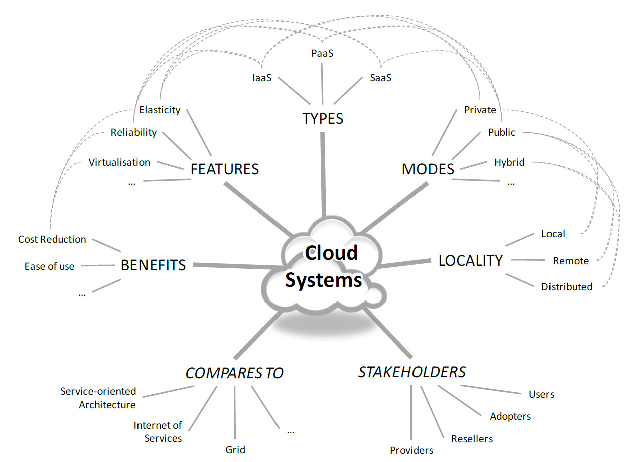
\includegraphics[width=8cm, height=7cm]{Images/Non-Exhaustive-view-on-the-main-aspects-forming-a-Cloud-System-3.jpg}
  }{}
  \caption{Non-Exhaustive view on the main aspects forming a Cloud System adopted from \citeauthor{thiel2015cloud} (\citeyear{thiel2015cloud}) \cite{thiel2015cloud}}
  \label{fig: cloud_Systems}
\end{figure}

%\subsection{Types of Cloud}\label{subsection:cloud_types}

%\subsubsection{1. Private Cloud}\label{subsection:private_cloud}

%\subsubsection{2. Public Cloud}\label{subsection:public_cloud}

%\subsubsection{3. Community Cloud}\label{subsection:community_cloud}

%\subsubsection{4. Hybrid Cloud}\label{subsection:hybrid_cloud}

\subsection{Basic Cloud Computing Services}\label{subsection:computing_Services}
%\textit{Explain the basic cloud computing services based on definitions from different researches and reasons behind such definitions}
The major concept of Cloud computing is based on using distributed resources for application and services that need lots of computing assets for specific period in time \cite{khasnabish2012cloud}. Cloud computing is in general a kind of computing technique where these  services are provided by massive, low-cost computing units, connected by IP networks. A lot of big players in the software industry, along side companies known for their huge Internet technology like Google and Amazon have joined in the development and use of these cloud services \cite{armbrust2009above}, \cite{hilley2009cloud}, \cite{lin2009cloud}. Businesses that are not technically oriented also want to explore possibilities and numerous business benefits of cloud computing services. These provided services can be in form of form  of  infrastructure,  platform,  or  software in  a  pay-as-you-go  model; giving the consumer power to decide what type of service and for how long does he/she needs this service.

Although there are several proposed cloud computing service models; Service-as-a-Service \cite{li2010intel}, Data-as-a-Service \cite{hilley2009cloud}, \cite{wang2010cloud}, Storage-as-a-Service \cite{hilley2009cloud}], it is generally possible to group these and other proposed models with the existing three service models, analogous to the technical layers in most cloud realizations: infrastructure, platform, and application.

%https://link.springer.com/content/pdf/10.1007%2Fs13174-011-0027-x.pdf
%https://link.springer.com/content/pdf/10.1007%2F978-3-642-34062-8_52.pdf


\subsubsection{1. Infrastructure-as-a-Service (IaaS)}
IaaS is the conveyance of computing resources such as processing, storage and networks as a service (for example Amazon EC2\footnote{Amazon Elastic Compute Cloud (Amazon EC2). http://aws.amazon.com/ec2}). Cloud users can deploy and run their own system and the software application using these resource. Rather than purchasing servers, software, datacenter space or network equipment, they instead buy those resources as a fully outsourced service on demand and like every other cloud service billed based on resources consumed\cite{kepes2010moving}. This makes room for companies to use a virtual infrastructure without the large-scale startup costs, IT personnel, and storage space needed to maintain local infrastructure.

It is expected according to \cite{kepes2011understanding} that any IaaS should allow resources to be distributed as a service and allow dynamic scaling of this service, while allowing allocation of a single piece of hardware to users.

\subsubsection{2. Platform-as-a-Service (PaaS)}
PaaS one of the key services of cloud computing \cite{khan2012cloud}, known as "Cloudware \cite{khan2012cloud} and defined by NIST as \textit{“The capability provided to the consumer is to deploy onto the cloud infrastructure consumer-created or acquired applications created using programming languages, libraries, services, and tools supported by the provider. The consumer does not manage or control the underlying cloud infrastructure including network, servers, operating systems, or storage, but has control over the deployed applications and possibly configuration settings for the application-hosting environment”}. It provides a platform for users to directly develop their applications without worrying about hardware system set-up. PaaS supports the complete life cycle of an application \cite{SITARAM201273} with its major feature being that it supports all tenant applications with one code base. For reliability, availability, and security, conventional systems use security kernels and redundancy and rollback mechanisms, PaaS however leverages built-in testing, continuous validation, and automated triplicate writing and recovery as major techniques \cite{khan2012cloud}. It is based on an infrastructure that often has built-in, fault-tolerant facilities and supports scalable computing \cite{wang2010cloud}.

Although a PaaS solution provides a more restricted environment with fewer choices for operating systems and programming environments for its customers when compared to IaaS, it according to \cite{SITARAM201273}, nevertheless results in insignificant management burden on the customer.

Variety of cloud services can be hosted on a PaaS. It can be used by companies that want to host their application in a SaaS model without extra hardware or system software cost while benefiting from the flexibility of scaling to large number of users, they can also take advantage of the scale and availability while still maintaining security and privacy of data to deploy their applications in the cloud. PaaS systems can also be used by High Performance Computing applications and Internet-scale file hosting services; operations that require massive parallel computing.

Despite several advantages of PaaS, part of its downsides is that it is vendor locked-in and There is no standard cloud SDK or programming language \cite{teixeira2014building}. This means that once a decision is made on what SDK to use to for a feature changing vendors is not easy. The only way to change vendors at this moment is entirely redesign the part of the application that replies on the SDK functionality.

\subsubsection{3. Software-as-a-Service (SaaS)}
Software-as-a-service (SaaS) is one of three principal services of cloud computing. It run on top of IaaS and is generally an "all-ready" application that could range from business/company specific to general use applications, running on a cloud infrastructure like GAE\footnote{Google App Engine. http://code.google.com/appengine}, EC2 or Azure\footnote{Windows Azure. http://www.windowsazure.com}. SaaS service can have a huge number of tenants, with each tenant may have hundreds of thousands of users, and thus a SaaS infrastructure needs to supporting millions of users with scalable performance. The cost of the infrastructure, the right to use the application, hosting of the application, maintenance and support services are usually, depending on the payment option, all merged into a single monthly or per-use payment plan.

SaaS offers a variety of advantages over traditional software licensing models. Because the software does not live on the licensing company’s servers, there is less strain on the company to invest on new hardware. With SaaS users can access the software through a web browser from several locations in or outside the company/office. It is easy to implement, easy to update and debug, and can be less expensive (or at least have lower up-front costs) since users pay for SaaS as they go instead of purchasing multiple software licenses for multiple computers. SaaS costs great costs for SMEs, with low investment in hardware and its maintenance, which in general means low capital expenditure (on IT equipments) \cite{haselmann2011software}. \cite{haselmann2011software} also supports the argument that it has numerous uses including tracking leads, scheduling events, managing transactions, automating sign up, auditing and more, that are beneficial to also to SMEs.

While an SaaS service can be specified using service-oriented standards such as WSDL\footnote{Web Services Description Language (WSDL). https://www.w3.org/TR/wsdl20} or OWL-S \footnote{Semantic Markup for Web Services. https://www.w3.org/Submission/OWL-S}, it is important that its architecture addresses customization (the major challenge of SaaS \cite{sun2007software}), Multi-tenancy Architecture (MTA) scalability and rapid development.

Data security and speed of delivery are part of the draw back of SaaS. Because data for SaaS is stored on external servers, users of SaaS have to be sure that it is safe and cannot be accessed by unauthorized parties. Slow Internet connections can also impair performance, especially if the cloud servers are being accessed from locations where the internet connection is bad or accessed from afar off distances as internal networks tend to be faster than internet connections \cite{tsai2014software}.

\begin{figure}[h]
\centering
\IfFileExists{Images/CloudServices_Explained.png}{
    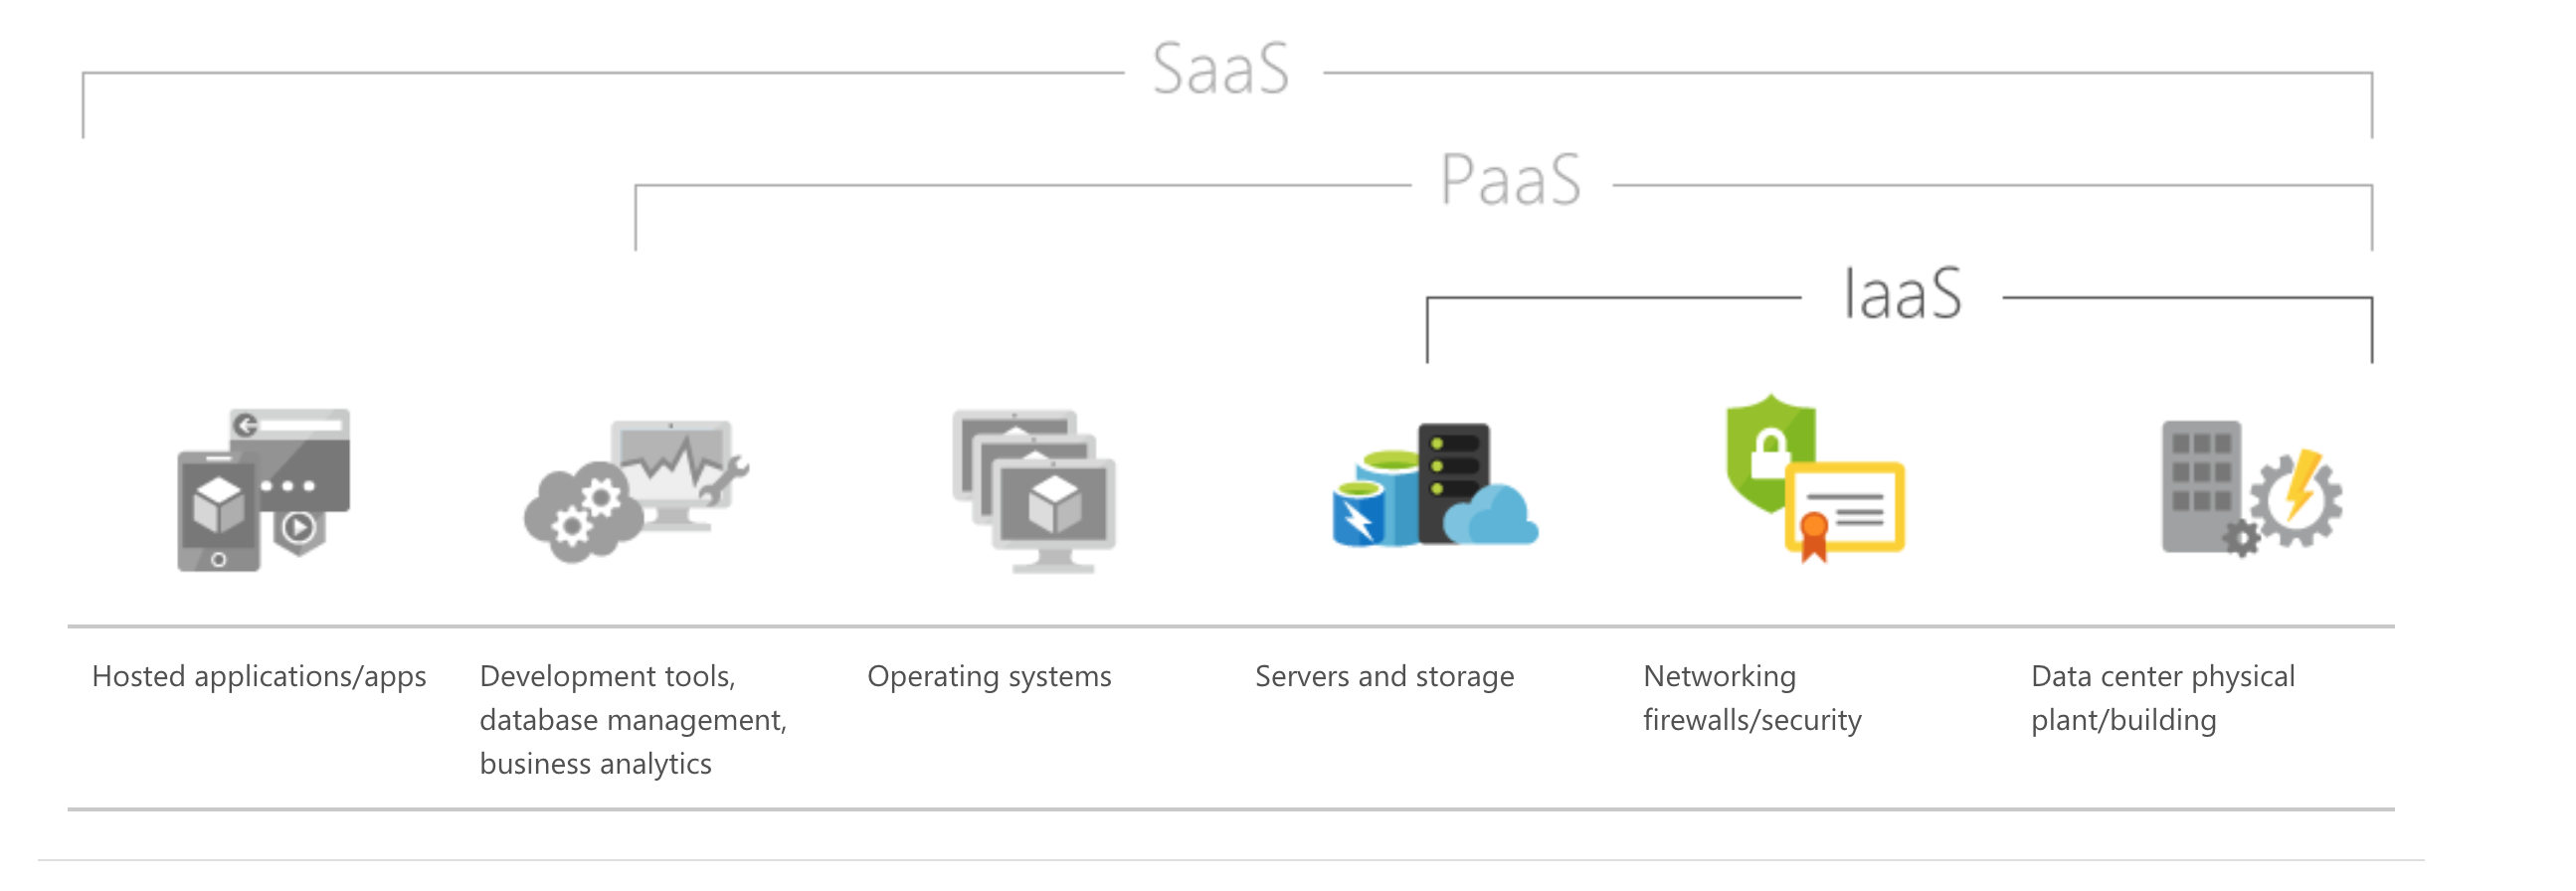
\includegraphics[width=12.5cm, height=5cm]{Images/CloudServices_Explained.png}
  }{}
  \caption{IaaS, PaaS, SaaS}
  \label{fig: cloud_services}
\end{figure}

\subsection{Architecture of Private Clouds} \label{subsection:arch._of_Private_Private_Cloud}
%\textit{Review the private cloud model and explain further including proposed architecture from different research. This is to give the reader insight on different possible adoptable private cloud architecture}
With cloud computing new computing paradigms have been introduced to IT organizations. At the same time, concerns are posed to it's users, such as security, privacy, data confidentiality, infrastructure control, and vendor lock-in. Due to this, the use of private and hybrid clouds become important alternatives for lots of cloud users. Using Private cloud nevertheless brings back IT management responsibilities, especially cloud operation management that cloud computing tries to eliminate \cite{doelitzscher2011private} back to the organization that choose to use a private cloud.

According to the deployment style and service object, there are 3 types of clouds: private clouds, public clouds and hybrid clouds \cite{tanwer2010thin}. Private clouds are constructed by an enterprise or institution for their own use, aimed to provide most effective control of data, safety and service quality. Enterprises in Private Cloud control the infrastructures, and control how applications are deployed on it. Generally, private cloud is deployed in enterprise's data center which is located behind firewalls, and it can also be deployed in a safe hosting place. It is important that in provisioning private clouds an architecture that supports its proposed use and implements IaaS, PaaS, SaaS is taken into consideration.

In \cite{zheng2011design}, an architecture was proposed. This architecture was based on a four layer virtualization \cite{bouali2016virtualization} with the in-house data center at the bottom of the architecture. \citeauthor{zheng2011design} [\citeyear{zheng2011design}] prosed that in other to shield node faults and integrate all physical resources (servers, storages and network infrastructures) of data center into a relatively flexible resource pool, virtualization is to be used in the second layer. In their prosed architecture the cloud computing operation system was built above the virtualization level (second layer) as it will allow visual process management and dispatch of data center resources. Fourth layer of the architecture is database and middleware, database store all data from enterprise application system and middleware primarily provide general public parts which is abstracted from complex applications, in order to reduce the complexity of application development. The top is grid application layer. Enterprise applications are deployed here. This architecture is however best for Smart Grids private cloud or for private clouds that do not have intense security needs.

BlueSky architecture \cite{dong2009bluesky} proposed by \citeauthor{dong2009bluesky} is an architecture that used virtualization technology to expose hardware and middleware with fine detailing. These resources were virtualized as a resource pool but maintained and managed as a whole, while allowing real-time resources allocation. By using dynamic clustering during runtime applications are deployed into clusters. The BlueSky cloud framework monitors the real-time workloads of these applications, based on this, additional applications are automatically a added. With load balancing also introduced to this architecture, computation requests are routed according to real-time workloads. When disposing structured data, data fabric constructs distributed data caching on the basis of cloud distributed environment to boost accesses. The BlueSky architecture uses this method to deal with it distributed file system storage tasks. 

The BlueSky unlike the architecture proposed by \cite{zheng2011design} has Six layer with functions of each layer encapsulated in form of service by on the principle of SOA\footnote{SOA. https://www.tutorialspoint.com/soa}. With the User interface layer is the entry-point into BlueSky cloud, providing a functional interface and interaction interfaces, including Web UIs and clients. The application layer focuses on the logical presentation of processes. The Common service layer provides reusable common services for higher layers, such as provision services, monitoring services, information services, account management services, and log management services. Services are encapsulated from the components of the capability layer. Made up of core components; provision manager, monitoring, trigger, etc, the capacity layer provide specific types of capabilities that manage and maintain the resource pool in the virtual infrastructure layer. Traditional middleware are also provided in this layer, including load balancing and data caching component. The BlueSky has data information layer which provides functions of data fabric for persistence and manages the storage of VM images. Virtual infrastructure layer of BlueSky enhances the transparency of hardware by virtualization, and realizes fine-grained management of resources.

A private cloud with this kind of architecture according to \cite{dong2009bluesky} will allow organizations to build systems that allocate resources on demand, solving issues like dynamic workload allocation and system scalability and resource management while improving performance, availability and scalability but also like the architecture of \cite{zheng2011design} does not have a dedicated security layer to handle security challenges of today's cloud environment. 

\section{Private Cloud for Educational Institutions}\label{section:private_cloud}
%\textit{Since one of our objectives is to deploy a private cloud on an educational institutions server. I will review the use of private cloud for educational institutions here}
Currently, Learning systems for most educational institutions are still weak on scalability at the infrastructure level. Resources and physical machines of these learning systems are usually simply and exclusively stacked, most of which are deployed and assigned for only specific tasks or applications, and high workloads - something that is bound to always occur during the lecture period in these institutions, as projects and assignment will be carried out by a great number of student, are handled by simply adding new resources. Stacking resources to existing ones every time there is high workload is not the best solution. This makes these systems to often hold-on to resources in and out of peek periods, it leads to great overhead in resources and unacceptable increase in (management) cost.

Cloud computing infrastructure has provided tremendous possibilities to alleviate this issue, providing dynamically scalable infrastructure for storage, computation, communication capabilities as a service which education institutions can take advantage of.

\subsection{Private Cloud Architecture for Educational Institutions}
%\textit{Review different possible private cloud architectures used by different institutions while deploying their private cloud}
The architectures \cite{zheng2011design} and \cite{dong2009bluesky} mentioned in \textit{\ref{subsection:arch._of_Private_Private_Cloud}} are proposed for educational purposes but they both lack some required layers and components that are essential for proper functioning and security of a private cloud provisioned for education institutions. The virtual Computing Laboratory (VCL) \cite{vouk2008powered} developed by the North Carolina State University is an architecture that depicts what we are trying to develop in this work. The architecture was developed to server students and faculty members of North Carolina University and out-of-state Universities with population of users way over 30,000. This architecture maps well to cloud computing requirements and expectations, it gives room; for elements to be re-used by others, it allow for alternative implementations - very precisely; make specified interfaces available, make run-time components replacement mechanism available to user, provide ability to verify and validate substitutions changes. It provides ability to readily extend system component pool, increase capabilities of individual  components, have an extensible architecture that can automatically discover new functionalities and resources, etc). Ability to customize features to the needs of a particular domain as in this framework are made available to a certain group of users. Most importantly considering the number of users, the ability to scale solutions.

The VCL architecture abstracts resources at several levels both at hardware, application and operating systems (OS) level. It abstracts software from hardware and at user level it delivers a mixture of hardware and software abstraction, a user has either a sole use of one or more hardware units or shares resources with other users, they also have different rights with respect to what actions they are allowed to perform. User groups in this architecture include: \textbf{\textit{Manager}} - functions as the image loader and platform manager, basically allow to perform advanced user functions and the \textbf{\textit{User}} - this user basically makes use of the cloud services provided by VCL.
\begin{figure}[h]
\centering
\IfFileExists{Images/logical_Architecture_of_VCL.png}{
    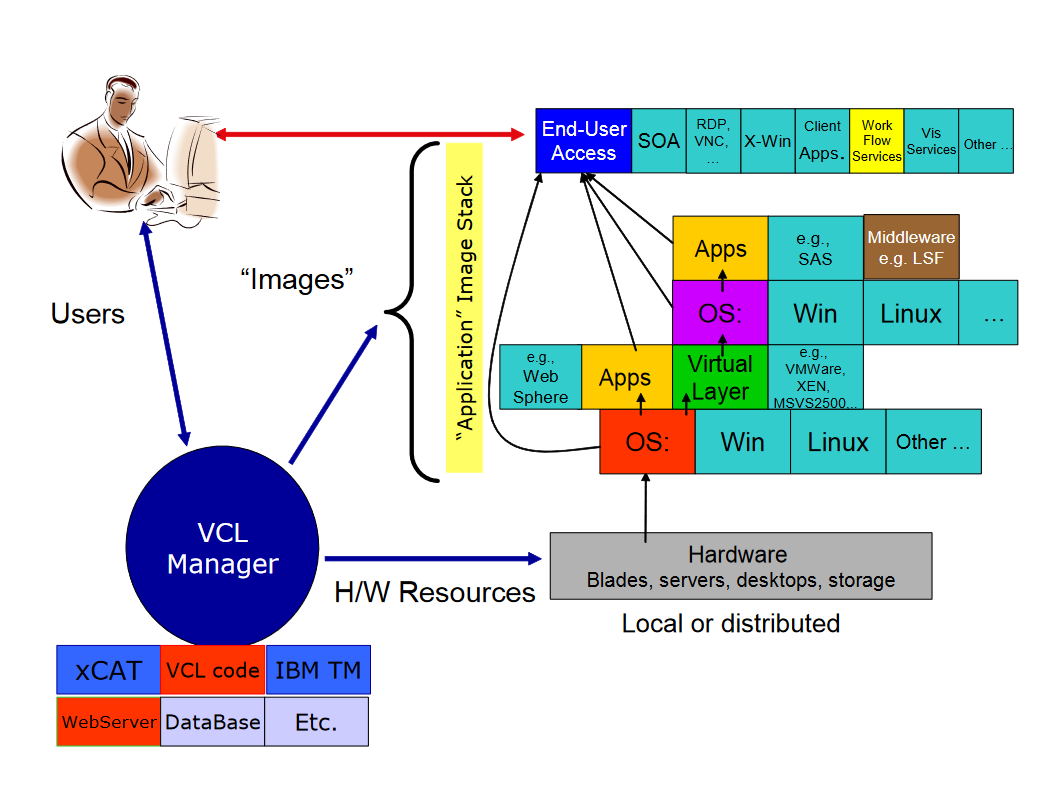
\includegraphics[width=12.5cm, height=8cm]{Images/logical_Architecture_of_VCL.png}
  }{}
  \caption{Illustration of the Logical Architecture of VCL \cite{vouk2008powered}}
  \label{fig: logical_Architecture_of_VCL}
\end{figure}

The VCL services is focused on controlling the resources at platform level, therefore incorporates solutions like Citrix\footnote{Critix. https://www.citrix.com/} and hyperviser-based implementations. For security, authentication is based on Light-Weight Direct Access Protocol (LDAP)\footnote{LDAP. https://ldap.com/basic-ldap-concepts/}, with environment authentication determined at image creation time. It also allows for other security methods like VPN’s, private VLAN’s, ssh-tunneling, etc. For monitoring resources, IBM Tivoli Monitoring\footnote{IBM Tivoli Monitoring. https://www.ibm.com/support/knowledgecenter/en/SSTFXA\_6.3.0/\\com.ibm.itm.doc\_6.3/welcome\_63.htm} was used.

They are both exemplary, hence our interest in them and will be reviewing them extensively in this section.

\subsection{OpenStack Private Cloud Vs Other Private Clouds}
    \textit{Review other private cloud deployment projects, OpenNebula, Eucalyptus and cloudStack by comparing them to OpenStack: Pros, Cons, differences, reported bottle necks }
    	\subsubsection{1. OpenStack Vs OpenNebula}
        \subsubsection{2. OpenStack Vs Eucalyptus}
        \subsubsection{3. OpenStack Vs CloudStack}    

\section{Auto-scaling in Cloud}
    \textit{give an overview of auto-scaling in cloud based on research papers}
    \subsection{Importance of auto-scaling in cloud}
    \textit{possible gains when cloud owners effectively implement auto-scaling of their cloud}
    \subsection{Issue with auto-scaling in cloud}
    \textit{discovered issues associated with auto-scaling in cloud }
    
    \section{Benchmarking in Cloud}
	\subsection{Introduction}
\textit{Give an overview of benchmarking}
	\subsection{Benchmarking approaches in cloud}
    \textit{Review the different reported benchmarking approaches in cloud, case studies and results, what should be kept in mind while benchmarking in cloud, characteristics of a good benchmark, encountered problems and proffered solutions}
    \subsection{Cloud Benchmarking tools}
    \textit{review different tools for benchmarking in cloud}
    \subsection{Cloud Benchmarking tools selection}
    \textit{Review some criteria for selecting a cloud benchmarking tool}
    \subsection{CloudSuite as a Cloud Benchmarking tool}
    \textit{review and discuss further the different benchmarking components of CloudSuite}